\documentclass[10pt,twocolumn,letterpaper]{article}

\usepackage{cvpr}
\usepackage{times}
\usepackage{epsfig}
\usepackage{graphicx}
\usepackage{amsmath}
\usepackage{amssymb}
\usepackage{algpseudocode}
\usepackage{algorithm}
\usepackage{booktabs}
% Include other packages here, before hyperref.

% If you comment hyperref and then uncomment it, you should delete
% egpaper.aux before re-running latex.  (Or just hit 'q' on the first latex
% run, let it finish, and you should be clear).
\usepackage[breaklinks=true,bookmarks=false]{hyperref}

\cvprfinalcopy % *** Uncomment this line for the final submission

\def\cvprPaperID{****} % *** Enter the CVPR Paper ID here
\def\httilde{\mbox{\tt\raisebox{-.5ex}{\symbol{126}}}}

% Pages are numbered in submission mode, and unnumbered in camera-ready
%\ifcvprfinal\pagestyle{empty}\fi
\setcounter{page}{1}
\begin{document}

%%%%%%%%% TITLE
\title{\LaTeX\ Author Guidelines for CVPR Proceedings}

\author{Chen Du\\
PID: \\
{\tt\small @eng.ucsd.edu}
% For a paper whose authors are all at the same institution,
% omit the following lines up until the closing ``}''.
% Additional authors and addresses can be added with ``\and'',
% just like the second author.
% To save space, use either the email address or home page, not both
\and
Wenjun Zhang\\
PID: A53218995\\
{\tt\small wez177@eng.ucsd.edu}
\and
Jingyi Yang\\
PID: A53216941\\
{\tt\small jiy349@eng.ucsd.edu}
\and
Jinzhao Feng\\
PID: \\
{\tt\small @eng.ucsd.edu}
}

\maketitle
%\thispagestyle{empty}

%%%%%%%%% ABSTRACT
\begin{abstract}
   Abstract here.
\end{abstract}

%%%%%%%%% BODY TEXT
\section{Introduction}

Introduction here.

%------------------------------------------------------------------------
\section{Gesture Recognition System}

We built our gesture recognition system which could recognize number gesture from one to five and show the corresponding numbers. This system is based on Matlab, which is one of the most popular computer vision platforms. The block diagram of the system is shown in figure.1.This system could be separate into 3 parts: detection, tracking and recognition.

\begin{figure}
     \centering
       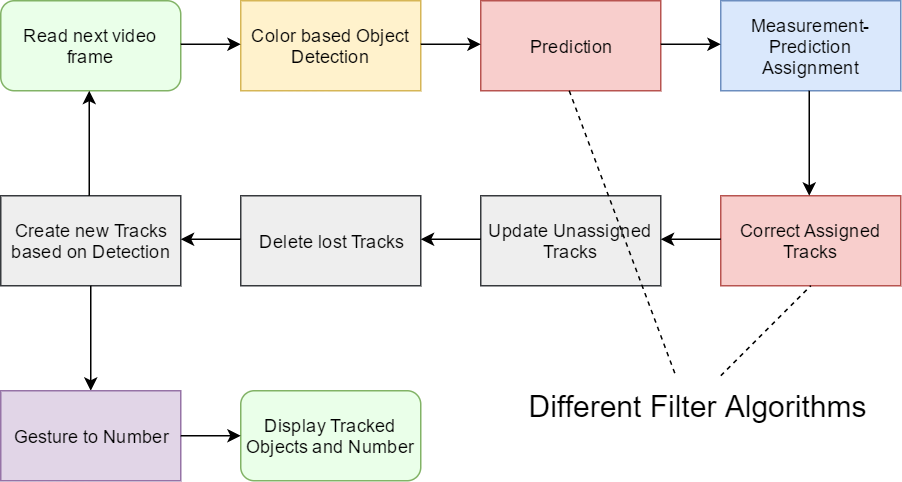
\includegraphics[width=0.5\textwidth]{duchen_1.png}
         \caption{\small{Diagram of Gesture Recognition System}}
 \end{figure}

\subsection{Object Detection}

We have tested 3 detection methods including correlation bases detection [1], foreground detection [2] and color-based detection [3]. Since the correlation-based object detection needs a specific template for each object and is unstable when object or lens rotates, it appeared low precision for finger detection where lots of rotations and random motions happen. Similarly, the foreground detection has a demand for fixed camera, and is hard to tell the fingers from non-target moving objects interference. Color-based detection is widely used in scenes where the objects have specific color, and has the advantage of robustness for moving object detection compared with other two methods. Using a glove with specific colored fingers, the color-based detection showed high precision and robustness. So we choose the color-based object detection to capture the fingers and hand locations. In detail, in each frame, the RGB value of each pixel <$r_x$, $g_x$, $b_x$> is compared with the target RGB value<$r_t$, $g_t$, $b_t$>, and the Euclidean norm of the difference is calculated as the distance:

\begin{equation}
dist_x=||r_x-r_t||+||g_x-g_t||+||b_x-b_t||\\
\end{equation}

If the distance is within a given threshold $dist_{th}$, this pixel is judged as target (foreground).

\begin{equation}
	target_x=
\begin{cases}
	1, & dist_x<dist_{th}\\
	0, & dist_x>dist_{th}
\end{cases}
\end{equation}

A mask of target is formed after all pixels have been judged. A blob analysis is performed on the mask and the finger-like connected components within given size will be output as the fingers and the centers are calculated as locations. Before blob analysis, we remove small connected components within a given area threshold (e.g. 100 pixels) to prevent false positive, then a morphologic closing is applied to remove the false negative holes caused by noise.

\subsection{Tracking}
We applied 4 kinds of filters which will be discussed in section 3. For multiple object tracking, one challenge is to correctly assign the predicted locations with the detected ones. Here we use the state-space distance [4] to compute the confidence.

\begin{equation}
d(z)=(z-Hx)^T\sum^{-1} (z-Hx)+ln|\Sigma|
\end{equation}

\begin{equation}
\Sigma=HPH^T+R
\end{equation}

In the above equations, z is the measurement and d(z) is the corresponding state-space distance, x is the predicted state, P is the state estimation error covariance, H is the measurement model, these metrics will be discussed in section 3. For each predicted state, we assign it to the measurement with lowest distance. For Kalman filters the assigned trackers will be corrected to get the tracked locations, while the unassigned trackers will just use predicted states as the tracked locations. For trackers which are unassigned for a certain number of continuous frames, we regard them as lost objects and delete them. For unassigned measurements new trackers will be created once they show up longer than a certain number of continuous frames.

\subsection{Convert Gesture to Number}

Once we have the tracked locations of the fingers and hand, we establish a 3x3 grid block based on hand location and count the finger numbers in each block, then output the corresponding meaning of the gesture, here the output contains numbers from 1-5. The connection between number count and the output is set manually, and is adjustable to add other meanings of gestures.

\begin{figure}
     \centering
       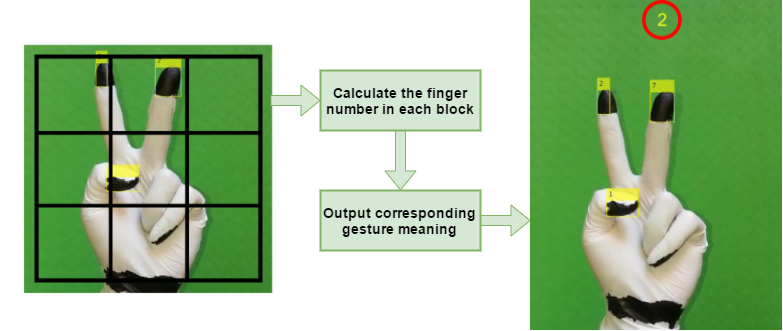
\includegraphics[width=0.5\textwidth]{duchen_2.png}
         \caption{\small{Gesture-to-number Conversion}}
 \end{figure}

%------------------------------------------------------------------------
\section{Filter Theory}

\subsection{Kalman Filter}

Kalman filter has been widely applied in object tracking. The Kalman filter is the optimal filter to estimate the state of a linear dynamic system when only noisy measurements are available[1]. Due to analytic tractability both operation and measurement noises are required to be Gaussian. In 1960, Ruodolf Kalman first introduced the system[2], and it was first applied in estimating the trajectory for the NASA Apollo program in 1969[3].

The operation of the filter basically consists of 2 steps:

1 Prediction, based on the last estimated state $\hat{x}_{k-1}$ and covariance matrix $P_{k-1}$:

\begin{equation}
\hat{x}_k^-=A\hat{x}_{k-1}+Bu_k
\end{equation}

\begin{equation}
P_k^-=AP_{k-1}A^T+Q
\end{equation}

where $A$ is the time-transition matrix,  $u_k$ is the control or external input, $B$ is a linear matrix which characterize the effects of the external input, and $Q$ is the operation noise covariance matrix.

Equation (1) predicts the most probable state $\hat{x}_k^-$ based on the last estimation and external input. Equation (2) predicts the new covariance matrix $P_k^-$ of the predicted state, given the previous estimated covariance matrix and operation noise.

2 Correction, based on the measurements to correct the prediction:

\begin{equation}
K_k=P_k^-H^T(HP_k^-H^T+R)^{-1}
\end{equation}

\begin{equation}
\hat{x}_k=\hat{x}_k^-+K_k(z_k-H\hat{x}_k^-)
\end{equation}

\begin{equation}
P_k=(I-K_kH)P_k^-
\end{equation}

where $K_k$ is the Kalman gain, the term $z_k-H\hat{x}_k^-$ is called the innovation, $H$ is the measurement matrix, and $R$ is the measurement noise covariance matrix.

The Kalman gain $K_k$ controls the effect that the current measurement has over the new state. Equation (4) and (5) correct the prediction based on the Kalman gain to estimate the state $\hat{x}_k$ and covariance matrix $P_k$.

Because the new estimations are generated based only on the previous state estimation and the current measurements, the Kalman filter is an online estimator. Besides, by increasing $Q$ and $R$, $P_k^-$ increases and $K_k$ tends to zero, meaning that the last state becomes less important and the new measurement becomes less effective. It should also be noted that the transition matrix $A$ and measurement matrix H in Kalman filter are certain, so when the model is non-linear, no such certain matrices $A$ and $H$ exist, and Kalman filter no longer works.

%-------------------------------------------------------------------------
\subsection{Extended Kalman Filter}

The Extended Kalman filter (EKF)[4][5] has been applied to alleviate the constraint of linearity. The basic framework of Extended Kalman filter is similar to that of Kalman filter, which is shown in Figure. 1. For convenience, the control input $u_k$ has been set to zero. What?s different is that the Extended Kalman filter uses the linear function $f$ and $h$ to linearize the nonlinear transformations for state prediction and predicted measurement. And the transition matrix $A$ and measurement matrix $H$ are substituted with Jacobian matrices derived from the non-linear function $f$ and $h$:

\begin{equation}
A=\frac{\partial f}{\partial x}|_{\hat{x}_{k-1}}
\end{equation}

\begin{equation}
H=\frac{\partial h}{\partial x}|_{\hat{x}_k^-}
\end{equation}

The reason why matrix $A$ is derived at the point $\hat{x}_{k-1}$ is that, compared to $\hat{x}_k^-$, the previous estimated state $\hat{x}_{k-1}$ is closer to reality so the matrix $A$ will better approximate the actual linearized model.

\begin{figure}
     \centering
       \includegraphics[width=0.5\textwidth]{pic_1.png}
         \caption{\small{Diagram Comparison between EKF and KF}}
 \end{figure}

The Jacobian matrix is obtained through the first order partial derivative, so the Extended Kalman Filter can be viewed as "first order" approximation to the optimal terms[6]. However, the Extended Kalman filter can introduce large errors when the high order terms cannot be overlooked. As shown in figure.2[7], linearized transformation is not reliable if propagation cannot be well approximated by a linear function[8], and actually the system may divergent. In addition, linearization can be applied only if the Jacobian matrices exists. Furthermore, the heavy computation of Jacobian matrices makes EKF impractical in many situations.

\begin{figure}
     \centering
       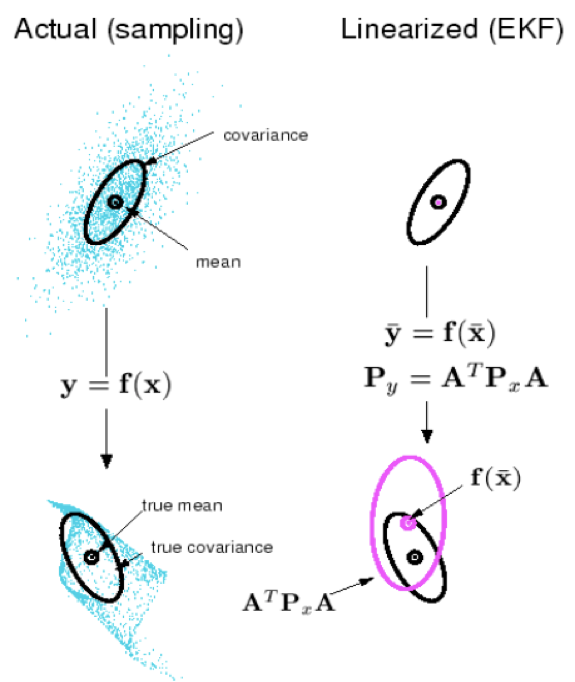
\includegraphics[width=0.4\textwidth]{pic_2.png}
        \caption{\small{Mean and Covariance Propagation}}
 \end{figure}

%-------------------------------------------------------------------------
\subsection{Unscented Kalman Filter}

The Unscented Kalman Filter[9], proposed by Julier and Uhlman, addresses the approximation issues of the Extended Kalman Filter. The intuition of this improvement is to approximate a probability distribution rather than a non-linear function. To achieve this, a set of points are carefully chosen to described the mean and covariance, and the points are called the sigma points[10].

The Unscented Kalman Filter can be seen as a combination of Unscented Transformation and Kalman Filter. We start first explaining the unscented transformation[11].

The unscented transformation(UT) is a method to compute the statistics of a random variable undergoing nonlinear transformation by transforming each sigma point through the nonlinear function. Suppose a random variable $x$ (dimension $n$) with mean $\mu$ and covariance matrix $
\sum$ is propagated through a nonlinear model with function $y=g(x)$. A matrix $X$ of $2n+1$ vectors $X_i$ is formed as the set of sigma points, and each vector is corresponding with weight $W_i$. The procedures are according to the following:

Choosing the sigma points

\begin{equation}
X^{[0]}=\mu
\end{equation}

\begin{equation}
X^{[i]}=\mu+(\sqrt{(n+\lambda)})_i for i=1, ..., n
\end{equation}

\begin{equation}
X^{[i]}=\mu+(\sqrt{(n+\lambda)})_{i-n} for i=n+1, ..., 2n
\end{equation}

Weights sigma points

\begin{equation}
w_m^{[0]}=\frac{\lambda}{n+\lambda}
\end{equation}

\begin{equation}
w_c^{[0]}=w_m^{[0]}+(1-\alpha^2+\beta)
\end{equation}

\begin{equation}
w_m^{[i]}=w_c^{[i]}=\frac{1}{2(n+\lambda)} for i=1, ..., 2n
\end{equation}

where $\lambda=\alpha^2(n+k)-n$ is a scaling parameter. $\alpha$ is usually set to small value and $k$ is usually set to zero, and both of them determine how far the sigma points are away from the mean. $\beta$ is used to incorporate prior knowledge of the distribution of $x$, and $\beta=2$ is the optimal choice for Gaussians. $(\sqrt{(n+\lambda)})_i$ is the $i$ th row of the matrix square root. These sigma vectors are propagated through the nonlinear model,

\begin{equation}
Y_i=g(X_i) for i=0, ..., 2n
\end{equation}

Therefore, the mean and covariance of y can be approximated by the summation of the weighted sample mean and covariance of the transformed sigma points,

\begin{equation}
\mu^{'}=\sum_{i=0}^{2n}w_m^{[i]}g(X^{[i]})
\end{equation}

\begin{equation}
\sum^{'}=\sum_{i=0}^{2n}w_c^{[i]}(g(X^{[i]})-\mu^{'})(g(X^{[i]})-\mu^{'})^T
\end{equation}

These sigma points completely capture the true mean and covariance accurately to the 3rd order for any nonlinearity. As shown in Figure.3[7], the right plots show the performance of the UT when using 5 sigma points. It?s obvious that the UT outperforms the other two methods, and it?s a better approximation than EKF for nonlinear models.

\begin{figure}
     \centering
       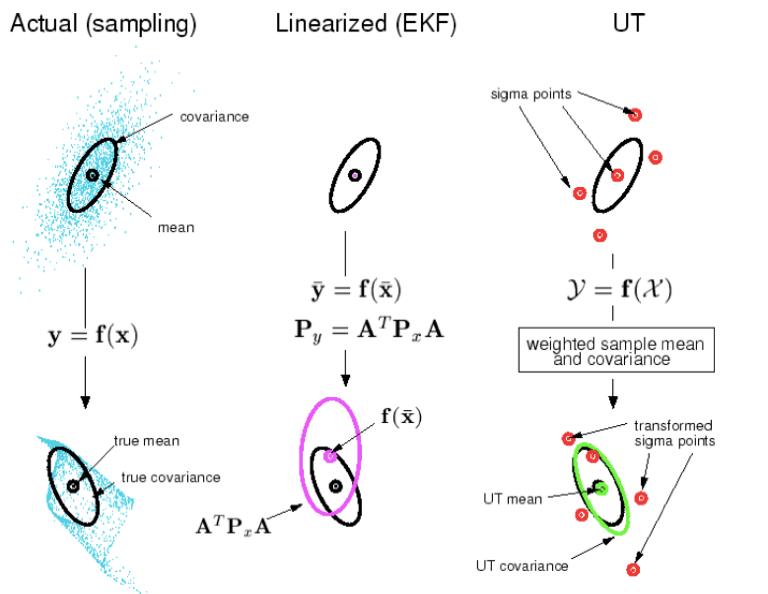
\includegraphics[width=0.5\textwidth]{pic_3.png}
        \caption{\small{Mean and Covariance Propagation}}
 \end{figure}

Therefore, when the mean and covariance of the input are certain, the mean and covariance of the non-linear transformation can be computed using UT. The algorithm of Unscented Kalman Filter is shown in Algorithm 1: Unscented Kalman Filter Algorithm. The basic framework is the same as the Extended Kalman Filter. The difference is that, instead of using the nonlinear functions directly for prediction and the Jacobian matrices to linearize the model, the Unscented Kalman Filter applies the UT to obtain the mean and covariance of the nonlinear propagation[12], so it does not require the computation of the Jacobian matrices.
\begin{algorithm}
\caption {Unscented Kalman Filter Algorithm}
\begin{algorithmic} [1]
\State  $Unscented\quad Kalman\quad Filter(\mu_{t-1},\quad \Sigma_{t-1},\quad u_t,\quad z_t)$
\State $\chi_{t-1}=(\mu_{t-1} \quad \mu_{t-1}+\sqrt{(n+\lambda)\Sigma_{t-1}} \quad \mu_{t-1}-\sqrt{(n+\lambda)\Sigma_{t-1}})$
\State $\bar\chi_t^*=g(u_t,\chi_{t-1})$
\State $\bar\mu_t=\sum_{i=0}^{2n} \omega_m^{[i]}\bar\chi_t^{*[i]}$
\State $\bar\Sigma_t=\sum_{i=0}^{2n} \omega_c^{[i]}(\bar\chi_t^{*[i]}-\bar\mu_t)(\bar\chi_t^{*[i]}-\bar\mu_t)^T+R_t$
\State $\bar\chi_t=(\bar\mu_t\quad \bar\mu_t+\sqrt{(n+\lambda)\bar\Sigma_t}\quad \bar\mu_t-\sqrt{(n+\lambda)\bar\Sigma_t})$
\State $\bar{Z}_t=h(\bar\chi_t)$
\State $\hat{z}_t=\sum_{i=0}^{2n} \omega_m^{[i]}\bar{Z}_t^{[i]}$
\State $S_t=\sum_{i=0}^{2n}  \omega_c^{[i]} (\bar{Z}_t^{[i]}-\hat{z}_t) (\bar{Z}_t^{[i]}-\hat{z}_t)^T+Q_t$
\State $\bar\Sigma_t^{x,z}=\sum_{i=0}^{2n} \omega_c^{[i]}(\bar\chi_t^{[i]}-\bar\mu_t)(\bar{Z}_t^{[i]}-\hat{z}_t)^T$
\State $K_t=\bar\Sigma_t^{x,z}S_t^{-1}$
\State $\mu_t=\bar\mu_t+K_t(z_t-\hat{z}_t)$
\State $\Sigma_t=\bar\Sigma_t-K_tS_tK_t^T$
\State $return\quad \mu_t,\Sigma_t$
\end{algorithmic}
\end{algorithm}

Though no Jacobian matrices are needed, the Unscented Kalman Filter belongs to the same complexity class with the Extended Kalman Filter. Besides, the Unscented Kalman Filter is still restricted to Gaussian distributions.

%-------------------------------------------------------------------------
\subsection{Particle Filter}

Another popular tool in object tracking is the Particle Filter[13]. The Particle Filter method, first introduced by Gordon in 1993, is an efficient method to apply simulation for estimating unknown probability distributions, and it?s also known as sequential Monte Carlo method[14]. The Particle Filter is suitable in all kinds of frameworks, regardless of whether the model is linear or whether the noise is Gaussian. 

The basic idea of the algorithm is that any distribution can be represented as a weighted particle set, consisting of pairs $<x_k^{(i)}, w_k^{(i)}>$, where $x_k^{(i)}$ is a possible value of the system state and $w_k^{(i)}$ is its plausibility. Figure.5 indicates the diagram of particle filter. In particle filtering we first randomly generate a set of particle that represents the initial distribution. The posterior distribution is defined by a new particle set and it?s determined by a function $f$, which describes the dynamics of the system. The measurement update step is achieved by setting the weights according to the measurement data. The relation between the measurement data and the latent states is given by the conditional $h$. The most probably estimated state will be:

\begin{equation}
x_k=\sum_{i=1}x_k^{-(i)}w_k^{(i)}
\end{equation}

\begin{figure}
     \centering
       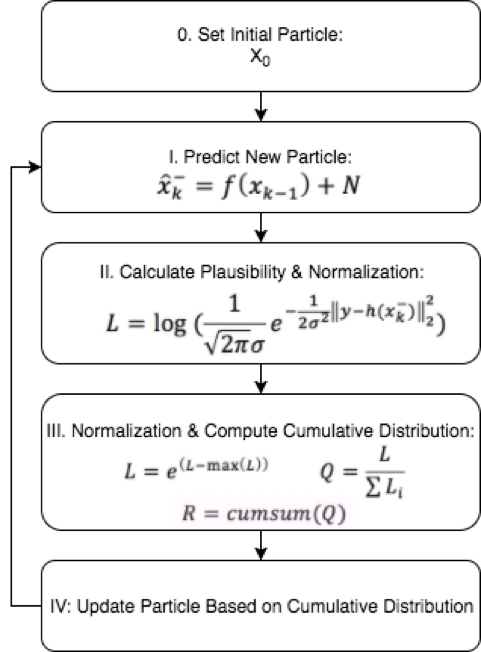
\includegraphics[width=0.3\textwidth]{pic_5.png}
        \caption{\small{Diagram of Particle Filter}}
 \end{figure}

It frequently occurs that almost all weights are zero except for one which tends to be one when implementing the Particle Filter in its basic form. To eliminate the effect, the resampling[15] is very important. The distribution can be updated as the particles be resampled with the weights which we obtain from the measurement data, as shown in Figure.6.

\begin{figure}
     \centering
       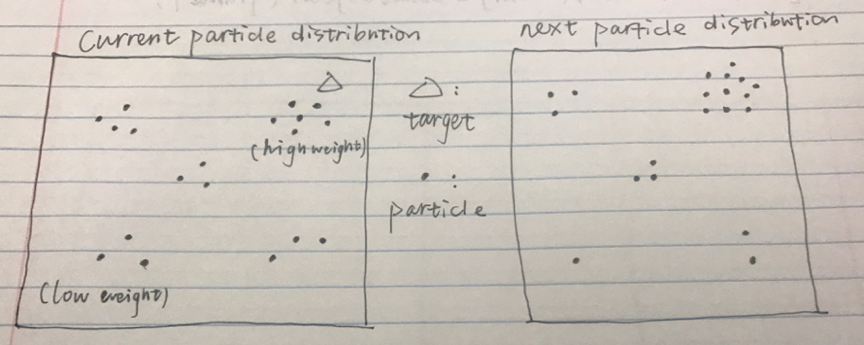
\includegraphics[width=0.5\textwidth]{pic_6.png}
        \caption{\small{Particles Resampling}}
 \end{figure}

When used in object tracking, the Particle Filter is usually applied with color detection and it?s relatively easy to implement. However, since the information of a pixel is just RBG information, it cannot work for gray-scale video, and its precision decreases sharply for low-light and occluded objects. Another issue is the decision of the sample size for adequate performance. An efficient set size has been introduced by Kong and Liu[15], which can be obtained from the weights of the particles following the equation below:

\begin{equation}
N_{eff}=\frac{N_s}{1+var(w_k)}
\end{equation}

where $N_s$ is the original set size. Notice that $N_{eff}<=N_s$, and small $N_{eff}$ indicates severe degeneracy, which is an undesirable effect in particle filters. A direct way to reduce this effect is to use very large $N_s$. So sufficient amounts of particles are prerequisite to ensure accurate tracking, and it can require high computation load for large-size video.

%-------------------------------------------------------------------------
\section{Experiment Design and Results}

To investigate the performances of different filters and confirm the hypothesis, we use the detection and tracking parts of our system to do a quantitative evaluation experiment, which aims to compare the tracking using different filters in various scenarios.

\subsection{Scenario Selection}

Considering factors which could affect the tracking performances, we design and record videos in scenarios shown below:
1) Linear motion model: the objects perform simple linear motion, e.g. straight line motion. Note there is no perfect linear motion in real life, so the linear motion is actually approximately linear motion. Despite small vibration or disturbance, the movement in a short period of continuous frame could be regarded as linear.
2) Nonlinear motion model: the objects perform mostly random motion, e.g. hand doing random gestures. It?s hard or impossible to manually calculate the state transition model in this case.
3) Occluded objects: objects are usually occluded in real life videos. A robust tracker should be able to handle the occlusion. In this kind of videos, objects are occluded partially or entirely in some frames, the occluded frame ratio varies from 10\% to 50\%.
4) Low-light condition: light is a very important factor that could influence the detection results. In this condition, objects moves in low-light environment which makes it hard to tell the target color for each pixel.
By choosing one of 2 motion models and one of 3 interferences (no interference is one choice), we have 6 combinations of scenarios.

\subsection{Evaluation Metric}

Many metrics for quantitative evaluation of target tracking have been proposed by researchers [5][6][7]. Since we focus on the tracking performance comparison, the precision plot which is used in recent year tracking benchmarks [8][9] is a suitable choice. The precision of a tracker means the percentage of frames whose estimated location is within the given threshold distance of the ground truth [8]. We are able to see the tracking performances with different error tolerances from precision plot directly.

\subsection{Parameters}

The system parameters are shown in Table. 1, for different trackers and videos, the noise value is selected based on the scenario. When the detector works well, i.e. there is enough light and no occlusion, the measurement noise is set to low value, while in low-light or occluded conditions, the measurement noise is set to high value. The motion noise is based on the goodness-of-fit of transition matrix/function to the motion model, for Kalman filter and Particle filter, motion noise is set to high for complex motion, and low for simple motion.

\begin{table}[h!]
  \centering
  \caption{System Parameters}
  \label{tab:table1}
  \begin{tabular}{|c|c|}
    \toprule
    \textbf{System Parameter} & \textbf{Value}  \\ \hline
    \midrule
  Motion Noise & 10 to 1000  \\ \hline
    Measurement Noise & 10 to 10,000  \\ \hline
    Video(Frame) Size & 486x864  \\ \hline
    Frame Per Second & 12  \\ 
    \bottomrule
  \end{tabular}
\end{table}

The filter parameters are shown in Table 2. As has been discussed, the performance of three kinds of Kalman filters depends on the correct transition matrix/function, but for most non-linear motion, there is no general model to calculate transition function for EKF and UKF. To estimate the transition function of the hidden motion model, we assume the state of the target is approximately an autoregressive process:

\begin{equation}
x_k \approx f(x_{k-1},w)+v_k
\end{equation}

Using labelled ground truth, a feedforward neural network is applied to get the estimation of the transition function f(parameterized by w). The residual error after convergence was taken to be the motion noise. We apply particle filters with 3 amounts of particles with linear transition function.



%-------------------------------------------------------------------------
\section{Conclusion}

Conclusion here

%------------------------------------------------------------------------

\begin{thebibliography}{1}
\bibitem{Botond A. Bocsi, Lehel Csato} Botond A. Bocsi, Lehel Csato. Visual Tracking with Filtering Algorithms.
 \emph{2008 4th International Conference on Intelligent Computer Communication and Processing}, pages: 269-274, 2008.

\bibitem{R. E. Kalman} R. E. Kalman. A new approach to linear filtering and prediction problems.
 \emph{Transactions of the ASME?Journal of Basic Engineering}, 82(Series D): 35?45, 1960.

\bibitem{M. S. Grewal and A. P. Andrews} Botond A. Bocsi, Lehel Csato. Visual Tracking with Filtering Algorithms.
 \emph{M. S. Grewal and A. P. Andrews. Kalman Filtering: Theory and Practice Using MATLAB}, John Wilney and Sons, Inc., second edition, 2001.

\bibitem{Peter S. Maybeck} Peter S. Maybeck. Stochastic Models, Estimation, and Control.
 \emph{Mathematics in Science and Engineering}, Academic Press, Inc., vol.141, 1979.

\bibitem{H. W. Sorenson} H. W. Sorenson. Kalman Filtering: Theory and Application.
 \emph{Piscataway, NJ: IEEE}, 1985.

\bibitem{E. A. Wan, R. Van Der Merwe.} E. A. Wan, R. Van Der Merwe. The Unscented Kalman Filter for Nonlinear Estimation.
 \emph{Proceedings of the IEEE 2000 Adaptive Systems for Signal Processing, Communications and Control Symposium}, pages: 153-158, 2000.

\bibitem{Cyrill Stachniss} Cyrill Stachniss. Unscented Kalman Filter.

 \emph{http://ais.informatik.uni-freiburg.de/teaching/ws13/mapping/pdf/slam06-ukf-4.pdf}

\bibitem{Ye Yuan, Guiyuan Fu and Weirong Zhang} Ye Yuan, Guiyuan Fu and Weirong Zhang. Extended and Unscented Kalman Filters for Parameter Estimation of a Hydrodynamic Model of Vessel.
 \emph{2016 35th Chine Control Conference(CCC)}, pages: 2051-2056, 2016

\bibitem{S . J. Julier and J. K. Uhlmann} S . J. Julier and J. K. Uhlmann. Visual Tracking with Filtering Algorithms.
 \emph{2Proc. of AeroSense: The 11th Int. Symp. on Aerospace/Defence Sensing, Simulation and Controls}, 1997.

\bibitem{Ryan Turner and Carl Edward Rasmussen} Ryan Turner and Carl Edward Rasmussen. Model based learning of sigma points in unscented Kalman filtering.
 \emph{Machine Learning for Signal Processing(MLSP), 2010 IEEE International Workshop}, 2010.

\bibitem{S. J. Julier and J. K. Uhlmann} S. J. Julier and J. K. Uhlmann. Unscented filtering and nonlinear estimation.
 \emph{Preceedings of the IEEE}, vol.92, no.3, pages: 401-422, 2004.

\bibitem{Fredrik Gustafsson and Gustaf Hendeby} Fredrik Gustafsson and Gustaf Hendeby. Some Relations Between Extended and Unscented Kalman Filters.
 \emph{EEE Transactions on Signal Processing}, vol.60, no.2. pages: 545-555, 2012.

\bibitem{N. Gordon, J. Salmond, and A. Smith} N. Gordon, J. Salmond, and A. Smith. A Novel Approach to Non-linear/Non-Gaussian Bayesian State Estimation.
 \emph{IEEE Preceedings on Radar and Signap Processing}, pages: 107? 113, 1993.

\bibitem{C. P. Robert and G. Casella} C. P. Robert and G. Casella. Monte Carlo Methods.
 \emph{Springer}, second edition, 2004.

\bibitem{A. Doucet, S. Godsill, and C. Andrieu} A. Doucet, S. Godsill, and C. Andrieu. On Sequential Monte Carlo Sampling Methods for Bayesian filtering.
 \emph{Statistics and Computing}, vol.10, no.3, pages:197?208, 2005.
\end{thebibliography}

\end{document}
